
%% ksnavely_mjdb.tex
%% 2013
%% by Kyle Snavely
%%

% Note that the a4paper option is mainly intended so that authors in
% countries using A4 can easily print to A4 and see how their papers will
% look in print - the typesetting of the document will not typically be
% affected with changes in paper size (but the bottom and side margins will).
% Use the testflow package mentioned above to verify correct handling of
% both paper sizes by the user's LaTeX system.
%
% Also note that the "draftcls" or "draftclsnofoot", not "draft", option
% should be used if it is desired that the figures are to be displayed in
% draft mode.
%
\documentclass[journal]{IEEEtran}
%
% If IEEEtran.cls has not been installed into the LaTeX system files,
% manually specify the path to it like:
% \documentclass[journal]{../sty/IEEEtran}

% Some very useful LaTeX packages include:
% (uncomment the ones you want to load)


% *** MISC UTILITY PACKAGES ***
%
%\usepackage{ifpdf}
% Heiko Oberdiek's ifpdf.sty is very useful if you need conditional
% compilation based on whether the output is pdf or dvi.
% usage:
% \ifpdf
%   % pdf code
% \else
%   % dvi code
% \fi
% The latest version of ifpdf.sty can be obtained from:
% http://www.ctan.org/tex-archive/macros/latex/contrib/oberdiek/
% Also, note that IEEEtran.cls V1.7 and later provides a builtin
% \ifCLASSINFOpdf conditional that works the same way.
% When switching from latex to pdflatex and vice-versa, the compiler may
% have to be run twice to clear warning/error messages.

% *** CITATION PACKAGES ***
%
\usepackage{cite}
% cite.sty was written by Donald Arseneau
% V1.6 and later of IEEEtran pre-defines the format of the cite.sty package
% \cite{} output to follow that of IEEE. Loading the cite package will
% result in citation numbers being automatically sorted and properly
% "compressed/ranged". e.g., [1], [9], [2], [7], [5], [6] without using
% cite.sty will become [1], [2], [5]--[7], [9] using cite.sty. cite.sty's
% \cite will automatically add leading space, if needed. Use cite.sty's
% noadjust option (cite.sty V3.8 and later) if you want to turn this off
% such as if a citation ever needs to be enclosed in parenthesis.
% cite.sty is already installed on most LaTeX systems. Be sure and use
% version 4.0 (2003-05-27) and later if using hyperref.sty. cite.sty does
% not currently provide for hyperlinked citations.
% The latest version can be obtained at:
% http://www.ctan.org/tex-archive/macros/latex/contrib/cite/
% The documentation is contained in the cite.sty file itself.

% *** GRAPHICS RELATED PACKAGES ***
%
\ifCLASSINFOpdf
   \usepackage[pdftex]{graphicx}
  % declare the path(s) where your graphic files are
  % \graphicspath{{../pdf/}{../jpeg/}}
    \graphicspath{{.}}
  % and their extensions so you won't have to specify these with
  % every instance of \includegraphics
    \DeclareGraphicsExtensions{.eps}
\else
  % or other class option (dvipsone, dvipdf, if not using dvips). graphicx
  % will default to the driver specified in the system graphics.cfg if no
  % driver is specified.
   \usepackage[dvips]{graphicx}
  % declare the path(s) where your graphic files are
   \graphicspath{{.}}
  % and their extensions so you won't have to specify these with
  % every instance of \includegraphics
   \DeclareGraphicsExtensions{.eps}
\fi
% graphicx was written by David Carlisle and Sebastian Rahtz. It is
% required if you want graphics, photos, etc. graphicx.sty is already
% installed on most LaTeX systems. The latest version and documentation
% can be obtained at: 
% http://www.ctan.org/tex-archive/macros/latex/required/graphics/
% Another good source of documentation is "Using Imported Graphics in
% LaTeX2e" by Keith Reckdahl which can be found at:
% http://www.ctan.org/tex-archive/info/epslatex/
%
% latex, and pdflatex in dvi mode, support graphics in encapsulated
% postscript (.eps) format. pdflatex in pdf mode supports graphics
% in .pdf, .jpeg, .png and .mps (metapost) formats. Users should ensure
% that all non-photo figures use a vector format (.eps, .pdf, .mps) and
% not a bitmapped formats (.jpeg, .png). IEEE frowns on bitmapped formats
% which can result in "jaggedy"/blurry rendering of lines and letters as
% well as large increases in file sizes.
%
% You can find documentation about the pdfTeX application at:
% http://www.tug.org/applications/pdftex

% *** MATH PACKAGES ***
%
%\usepackage[cmex10]{amsmath}
% A popular package from the American Mathematical Society that provides
% many useful and powerful commands for dealing with mathematics. If using
% it, be sure to load this package with the cmex10 option to ensure that
% only type 1 fonts will utilized at all point sizes. Without this option,
% it is possible that some math symbols, particularly those within
% footnotes, will be rendered in bitmap form which will result in a
% document that can not be IEEE Xplore compliant!
%
% Also, note that the amsmath package sets \interdisplaylinepenalty to 10000
% thus preventing page breaks from occurring within multiline equations. Use:
%\interdisplaylinepenalty=2500
% after loading amsmath to restore such page breaks as IEEEtran.cls normally
% does. amsmath.sty is already installed on most LaTeX systems. The latest
% version and documentation can be obtained at:
% http://www.ctan.org/tex-archive/macros/latex/required/amslatex/math/

% *** SPECIALIZED LIST PACKAGES ***
%
%\usepackage{algorithmic}
% algorithmic.sty was written by Peter Williams and Rogerio Brito.
% This package provides an algorithmic environment fo describing algorithms.
% You can use the algorithmic environment in-text or within a figure
% environment to provide for a floating algorithm. Do NOT use the algorithm
% floating environment provided by algorithm.sty (by the same authors) or
% algorithm2e.sty (by Christophe Fiorio) as IEEE does not use dedicated
% algorithm float types and packages that provide these will not provide
% correct IEEE style captions. The latest version and documentation of
% algorithmic.sty can be obtained at:
% http://www.ctan.org/tex-archive/macros/latex/contrib/algorithms/
% There is also a support site at:
% http://algorithms.berlios.de/index.html
% Also of interest may be the (relatively newer and more customizable)
% algorithmicx.sty package by Szasz Janos:
% http://www.ctan.org/tex-archive/macros/latex/contrib/algorithmicx/

% *** ALIGNMENT PACKAGES ***
%
%\usepackage{array}
% Frank Mittelbach's and David Carlisle's array.sty patches and improves
% the standard LaTeX2e array and tabular environments to provide better
% appearance and additional user controls. As the default LaTeX2e table
% generation code is lacking to the point of almost being broken with
% respect to the quality of the end results, all users are strongly
% advised to use an enhanced (at the very least that provided by array.sty)
% set of table tools. array.sty is already installed on most systems. The
% latest version and documentation can be obtained at:
% http://www.ctan.org/tex-archive/macros/latex/required/tools/

% IEEEtran contains the IEEEeqnarray family of commands that can be used to
% generate multiline equations as well as matrices, tables, etc., of high
% quality.

% *** SUBFIGURE PACKAGES ***
%\ifCLASSOPTIONcompsoc
%  \usepackage[caption=false,font=normalsize,labelfont=sf,textfont=sf]{subfig}
%\else
%  \usepackage[caption=false,font=footnotesize]{subfig}
%\fi
% subfig.sty, written by Steven Douglas Cochran, is the modern replacement
% for subfigure.sty, the latter of which is no longer maintained and is
% incompatible with some LaTeX packages including fixltx2e. However,
% subfig.sty requires and automatically loads Axel Sommerfeldt's caption.sty
% which will override IEEEtran.cls' handling of captions and this will result
% in non-IEEE style figure/table captions. To prevent this problem, be sure
% and invoke subfig.sty's "caption=false" package option (available since
% subfig.sty version 1.3, 2005/06/28) as this is will preserve IEEEtran.cls
% handling of captions.
% Note that the Computer Society format requires a larger sans serif font
% than the serif footnote size font used in traditional IEEE formatting
% and thus the need to invoke different subfig.sty package options depending
% on whether compsoc mode has been enabled.
%
% The latest version and documentation of subfig.sty can be obtained at:
% http://www.ctan.org/tex-archive/macros/latex/contrib/subfig/

% *** FLOAT PACKAGES ***
%
%\usepackage{fixltx2e}
% fixltx2e, the successor to the earlier fix2col.sty, was written by
% Frank Mittelbach and David Carlisle. This package corrects a few problems
% in the LaTeX2e kernel, the most notable of which is that in current
% LaTeX2e releases, the ordering of single and double column floats is not
% guaranteed to be preserved. Thus, an unpatched LaTeX2e can allow a
% single column figure to be placed prior to an earlier double column
% figure. The latest version and documentation can be found at:
% http://www.ctan.org/tex-archive/macros/latex/base/


%\usepackage{stfloats}
% stfloats.sty was written by Sigitas Tolusis. This package gives LaTeX2e
% the ability to do double column floats at the bottom of the page as well
% as the top. (e.g., "\begin{figure*}[!b]" is not normally possible in
% LaTeX2e). It also provides a command:
%\fnbelowfloat
% to enable the placement of footnotes below bottom floats (the standard
% LaTeX2e kernel puts them above bottom floats). This is an invasive package
% which rewrites many portions of the LaTeX2e float routines. It may not work
% with other packages that modify the LaTeX2e float routines. The latest
% version and documentation can be obtained at:
% http://www.ctan.org/tex-archive/macros/latex/contrib/sttools/
% Do not use the stfloats baselinefloat ability as IEEE does not allow
% \baselineskip to stretch. Authors submitting work to the IEEE should note
% that IEEE rarely uses double column equations and that authors should try
% to avoid such use. Do not be tempted to use the cuted.sty or midfloat.sty
% packages (also by Sigitas Tolusis) as IEEE does not format its papers in
% such ways.
% Do not attempt to use stfloats with fixltx2e as they are incompatible.
% Instead, use Morten Hogholm'a dblfloatfix which combines the features
% of both fixltx2e and stfloats:
%
% \usepackage{dblfloatfix}
% The latest version can be found at:
% http://www.ctan.org/tex-archive/macros/latex/contrib/dblfloatfix/


%\ifCLASSOPTIONcaptionsoff
%  \usepackage[nomarkers]{endfloat}
% \let\MYoriglatexcaption\caption
% \renewcommand{\caption}[2][\relax]{\MYoriglatexcaption[#2]{#2}}
%\fi
% endfloat.sty was written by James Darrell McCauley, Jeff Goldberg and 
% Axel Sommerfeldt. This package may be useful when used in conjunction with 
% IEEEtran.cls'  captionsoff option. Some IEEE journals/societies require that
% submissions have lists of figures/tables at the end of the paper and that
% figures/tables without any captions are placed on a page by themselves at
% the end of the document. If needed, the draftcls IEEEtran class option or
% \CLASSINPUTbaselinestretch interface can be used to increase the line
% spacing as well. Be sure and use the nomarkers option of endfloat to
% prevent endfloat from "marking" where the figures would have been placed
% in the text. The two hack lines of code above are a slight modification of
% that suggested by in the endfloat docs (section 8.4.1) to ensure that
% the full captions always appear in the list of figures/tables - even if
% the user used the short optional argument of \caption[]{}.
% IEEE papers do not typically make use of \caption[]'s optional argument,
% so this should not be an issue. A similar trick can be used to disable
% captions of packages such as subfig.sty that lack options to turn off
% the subcaptions:
% For subfig.sty:
% \let\MYorigsubfloat\subfloat
% \renewcommand{\subfloat}[2][\relax]{\MYorigsubfloat[]{#2}}
% However, the above trick will not work if both optional arguments of
% the \subfloat command are used. Furthermore, there needs to be a
% description of each subfigure *somewhere* and endfloat does not add
% subfigure captions to its list of figures. Thus, the best approach is to
% avoid the use of subfigure captions (many IEEE journals avoid them anyway)
% and instead reference/explain all the subfigures within the main caption.
% The latest version of endfloat.sty and its documentation can obtained at:
% http://www.ctan.org/tex-archive/macros/latex/contrib/endfloat/
%
% The IEEEtran \ifCLASSOPTIONcaptionsoff conditional can also be used
% later in the document, say, to conditionally put the References on a 
% page by themselves.


% *** PDF, URL AND HYPERLINK PACKAGES ***
%
%\usepackage{url}
% url.sty was written by Donald Arseneau. It provides better support for
% handling and breaking URLs. url.sty is already installed on most LaTeX
% systems. The latest version and documentation can be obtained at:
% http://www.ctan.org/tex-archive/macros/latex/contrib/url/
% Basically, \url{my_url_here}.


% *** Do not adjust lengths that control margins, column widths, etc. ***
% *** Do not use packages that alter fonts (such as pslatex).         ***
% There should be no need to do such things with IEEEtran.cls V1.6 and later.
% (Unless specifically asked to do so by the journal or conference you plan
% to submit to, of course. )


% correct bad hyphenation here
\hyphenation{}

% Neutrinoless beta beta
\def\znbb{0$\nu\beta\beta$}
% 2 nu beta beta
\def\tnbb{2$\nu\beta\beta$}
% electron
\def\elec{e$^{-}$}
% electron anti-neutrino
\def\elanu{$\bar{\nu}_{e}$}
% electron neutrino
\def\elnu{$\nu_{e}$}
% neutrinoless half life
\def\Tznbb{T$^{0\nu}_{1/2}$}
%Ge 76
\def\ge76{$^{76}$Ge}
\begin{document}
%
% paper title
% can use linebreaks \\ within to get better formatting as desired
% Do not put math or special symbols in the title.
\title{The \textsc{Majorana} Parts Tracking Database}
%
%
% author names and IEEE memberships
% note positions of commas and nonbreaking spaces ( ~ ) LaTeX will not break
% a structure at a ~ so this keeps an author's name from being broken across
% two lines.
% use \thanks{} to gain access to the first footnote area
% a separate \thanks must be used for each paragraph as LaTeX2e's \thanks
% was not built to handle multiple paragraphs
%

\author{Kyle~Snavely
\thanks{Manuscript received ; .}
\thanks{This work was primarily supported by DOE grants no. DE-FG02-97ER4104 and DE-FG02-97ER41033}}

% note the % following the last \IEEEmembership and also \thanks - 
% these prevent an unwanted space from occurring between the last author name
% and the end of the author line. i.e., if you had this:
% 
% \author{....lastname \thanks{...} \thanks{...} }
%                     ^------------^------------^----Do not want these spaces!
%
% a space would be appended to the last name and could cause every name on that
% line to be shifted left slightly. This is one of those "LaTeX things". For
% instance, "\textbf{A} \textbf{B}" will typeset as "A B" not "AB". To get
% "AB" then you have to do: "\textbf{A}\textbf{B}"
% \thanks is no different in this regard, so shield the last } of each \thanks
% that ends a line with a % and do not let a space in before the next \thanks.
% Spaces after \IEEEmembership other than the last one are OK (and needed) as
% you are supposed to have spaces between the names. For what it is worth,
% this is a minor point as most people would not even notice if the said evil
% space somehow managed to creep in.



% The paper headers
\markboth{IEEE Transactions On Nuclear Science,~Vol.~11, No.~4, December~2012}%
{Snavely \MakeLowercase{\textit{et al.}}: The \textsc{Majorana} Parts Tracking Database}
% The only time the second header will appear is for the odd numbered pages
% after the title page when using the twoside option.
% 
% *** Note that you probably will NOT want to include the author's ***
% *** name in the headers of peer review papers.                   ***
% You can use \ifCLASSOPTIONpeerreview for conditional compilation here if
% you desire.




% If you want to put a publisher's ID mark on the page you can do it like
% this:
%\IEEEpubid{0000--0000/00\$00.00~\copyright~2012 IEEE}
% Remember, if you use this you must call \IEEEpubidadjcol in the second
% column for its text to clear the IEEEpubid mark.



% use for special paper notices
%\IEEEspecialpapernotice{(Invited Paper)}




% make the title area
\maketitle

% As a general rule, do not put math, special symbols or citations
% in the abstract or keywords.
\begin{abstract}
The \textsc{Majorana} \textsc{Demonstrator} is an ultra-low background physics
experiment searching for the neutrinoless double-beta decay of \ge76.
Detecting neutrinoless double-beta decay requries extreme radiopurity of components
used in the experiment's construction.
The \textsc{Majorana} parts tracking database is an application which tracks
cosmogenic activation in materials and parts used to build the \textsc{Demonstrator}.
Tracking the location of parts as they are produced and shipped provides an estimate
of their exposure to cosmic radiation and 
an important quality assurance check during construction. A web application for data entry
and a radiation exposure calculator have been developed as tools for
achieving the extreme radiopurity required for this rare decay search.
\end{abstract}

% Note that keywords are not normally used for peerreview papers.
\begin{IEEEkeywords}
  Low Background, Neutrinoless Double-Beta Decay, Web 2.0, Application Software
\end{IEEEkeywords}

% For peer review papers, you can put extra information on the cover
% page as needed:
% \ifCLASSOPTIONpeerreview
% \begin{center} \bfseries EDICS Category: 3-BBND \end{center}
% \fi
%
% For peerreview papers, this IEEEtran command inserts a page break and
% creates the second title. It will be ignored for other modes.
\IEEEpeerreviewmaketitle

\section{Introduction}
\IEEEPARstart{D}{etecting} neutrinoless double-beta decay (\znbb) would prove that neutrinos are their own antiparticle,
demonstrate that lepton number is not conserved, and may provide insight into
the mass hiearchy of the neutrino family \cite{phillips_mj} \cite{mj_wilkerson} \cite{avignone_neutrinos}.
The \textsc{Majorana Demonstrator} is part of a phased approach towards a tonne-scale search for \znbb\ in \ge76, with
a background goal of $2.5\times10^{-4}$ counts $keV^{-1} t^{-1} y^{-1}$ \cite{mj_wilkerson} in the region of interest
around the \znbb\ signal at 2039 keV.
The \textsc{Demonstrator}'s extreme radiopurity requirements and low energy threshold also make it sensitive to a signal from dark
matter candidate particles known as Weakly Interacting Massive Particles (WIMPs).

Achieving this low background goal requires a multifaceted strategy including detector shielding, assembly in an ultra-clean environment,
careful materials screening, and a comprehensive parts tracking effort.
To minimize backgrounds from cosmic radiation the \textsc{Demonstrator} is located deep underground
at the 4850' level of the Sanford Underground Research Facility (SURF).
However, many parts need to be transported or stored above ground and are subject to
cosmogenic activation -- unstable isotopes in detector components created by cosmic radiation which may later decay and become background
to physics measurements.

Parts tracking is essential to realizing the \textsc{Demonstrator}'s background goal and controlling logistics.
Determining the activation rate of cosmogenic isotopes allows for an estimate of background
radiation originating from detector components. \textsc{Majorana} has developed a CouchDB  \cite{couchdb_guide} based 
parts tracking database (PTDB)
for tracking parts used in the construction of the experiment. The PTDB has a web-application frontend
for data entry and a Python based exposure calculator. The exposure calculator converts storage and transportation history 
into time and elevation profiles which can be used to estimate
material activity which can be folding into monte-carlo background simulations.

Tracking components also plays an important role in quality assurance during 
construction. A part's history (cleaning, transportation, etc...) must be 
understood before it can be integrated into production hardware. The information tracked
to benefit \textsc{Majorana}'s physics goals also greatly benefits conventional logistics in an
experiment which has thousands of individual components.

This paper begins by reviewing logistics for an ultra-low background
physics experiment, technologies used to create the web application, and
how our data is stored and queried. The final sections of the paper detail
the structure of the web application and exposure calculator as well as reflect
on the benefits of tracking part history for the \textsc{Demonstrator}.

\section{Parts Tracking}
When a part is created for the \textsc{Demonstrator}, it is given a unique serial number by the PTDB. The parent stock
is noted and material type inherited. Throughout the part's lifetime it receives history entries which range from storage
and transportation to processes which a part may undergo including cleaning, machining, and many others.

Detailed part histories will allow \textsc{Majorana}
to red-flag parts which may be excessively radioactive, allow for comprehensive background simulations,
or aid in troubleshooting if a source of background is found within the experiment.
Part history is also referenced during construction to ensure components meet quality requirements.

\subsection{Logistics Overview}

To uniquely identify parts and stock used by \textsc{Majorana} a serial number is laser engraved into metal and plastic parts.
Some parts are too large or small to be easily engraved, or are otherwise unsuitable for laser engraving, and these
components are identified by metal stamps or labels. Groups of small identical parts are bagged together
and a range of serial numbers is listed on the bag.

There are many materials used in the \textsc{Demonstrator}, but the bulk of the mass of the \textsc{Demonstrator}'s components is copper.
Steel, teflon, and other plastics are 
present in smaller amounts. Majorana electroforms the worlds purest copper in its undeground electroforming facility, also at SURF \cite{mj_wilkerson}.
This ultra-pure copper is visually indistinguishable from commercial copper and so material
tracking is vital.


\textsc{Majorana} manufactures its own detector components deep underground in its clean machine shop, and tracking the 
flow of stock material to finished parts is an important responsibility of the PTDB.
Thus, the stock and part relationship is also tracked
within the PTDB.  When a stock-part relationship is established (known generally as parent-child),
the child inherits the parent record's material type. 

The parent-child relationship is strictly one to many. No part can have more than one parent, as the parent-child link
represents a reducing process, such as machining parts or cutting cables. An object which is made from more than one individual
component is known as an assembly. The PTDB represents such relationships and provides each assembly with its own serial number. A part can be a member of only one assembly,
and an assembly may be a component of another assembly.

The assembly types in \textsc{Majorana} are drawn directly from the project engineering CAD designs and represent logical 
groupings of parts, such as Detector Units, Detector Strings, or Cryostats. 
Some assemblies contain multiple identical parts such as the three Hollow Hex Rods (custom copper bolts) in a Detector Unit.
Each Hollow Hex Rod is assigned a role number which correlates directly to the simulation geometry designed by \textsc{Majorana}. 

By assigning each part an indivdual position number, abberant backgrounds can be examined through positional analysis in 
simulation and the radioactive part identified without immediate deconstruction of an assembly, which is very costly in 
terms of manpower and time. During the assembly of detector components detailed notes are kept in physical logbooks that are
transcribed into an electronic logbook, and finally the assembly information is entered into the PTDB.

Given a serial number, one can examine a part in the PTDB and walk up the assembly tree. For example, the Hollow Hex Rod is a member
of a Detector Unit, which is a member of a Detector String, which is in turn a component of a Cryostat assembly.
If a history entry is applied to an assembly, it is also applied to each component or sub\-assembly in the assembly tree. If a Cryostat receives
a transportation history entry, each Detector String, Detector Unit, and Hollow Hex Rod currently in the tree will receive the same entry.

The are many types of history entries, including storage and transporation (which are used to estimate cosmogenic activation), machining, cleaning,
and others. A history entry references one or more locations which are stored in a document in the database. Each location has address meta-data
associated with it, and \textsc{Majorana}'s exposure calculation software uses the 
Google Maps Application Programming Interface (API) \cite{google_maps_dev_guide} to convert these addresses into latitudes, longtitudes, and elevations,
as well as provide sampled travel route information. The elevation versus time
profile is used to calculate an estimate of activation rates for cosmogenic isotopes in tracked components.

The machining process irreversibly changes a part's structure. Many subtle details may differentiate
two otherwise very similar looking parts. Tracking the machining date, machinist, and \textsc{Majorana} drawing number allows
for ambiguities to be resolved when a component's history is called into question. 

Components used by \textsc{Majorana} go through many processes. Cleaning, for instance, is a complicated task for an ultra-low
background experiment. There are many different cleaning processes a part may undergo and a part's cleaning history
must be understood before integration into detector hardware. For example, history entries stored alongside part records in the PTDB
allow scientists to verify whether a part has been acid etched, ultrasonic cleaned, or wiped with ethanol/isopropanol.

There are many other process types and not every type can
be accounted for during application development. As such, any user can 
easily add process types directly from the User Interface (UI). Some processes require an official \textsc{Majorana} procedure to be
followed and entry of the \textsc{Majorana} procedure number is required.

In addition to physics information provided by tracking material exposure to cosmic radiation, parts tracking also provides
a great logistics benefit to \textsc{Majorana}. Organizing and tracking information about thousands of components is a
challenge faced by many organizations. Providing a web interface for data entry and retrieval allows
a non-expert user to interact with data stored in \textsc{Majorana}'s CouchDB. Any web browser becomes a tool which can
be used to query information about part location or history.

\subsection{Database Record Structure}

\subsection{Parts Tracking Software Overview}
A JavaScript based web application frontend has been developed by \textsc{Majorana} as an easy-to-use tool for data-entry (see Fig. \ref{interface}).
Adopting modern programming techniques, using CouchDB, and leveraging libraries like JQuery and Backbone.js (see appendix for a complete list) allows the
web application to be easily extendable and maintainable throughout the project lifetime. Calculation of
activation rates is done with a small Python application which walks through data entered into the web
frontend and calculation results are pushed to the CouchDB database.

\begin{figure}[!t]
\centering
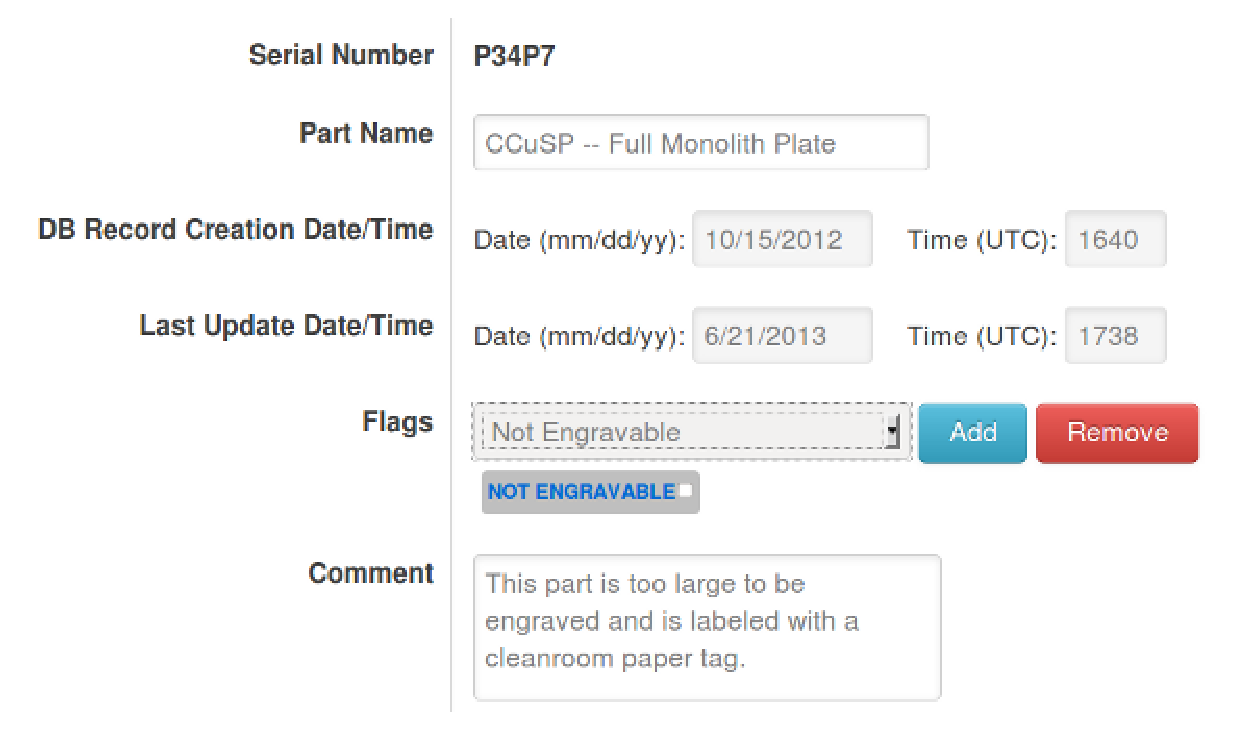
\includegraphics[width=3.5in]{interface}
\caption{A screenshot of the required forms of a part or assembly as presented to the user.
These DateFormView instances are disabled for input. The part has a ``Not Engravable" flag,
as it is too large to engrave. The CommentFormView expands when a user clicks on the text area.}
\label{interface}
\end{figure}

\subsubsection{JavaScript and Web Applications}
As both client computers and data-serving cloud power grow, the web browser has become a
platform for application development. Web applications and services are undergoing
a drastic departure from their humble beginnings \cite{ginige_web}. Web applications can be used by 
non-experts without the need for code management, compiling, or updating software. Technologies proven on the web such as HyperText Markup Language (HTML)
and JavaScript provide a graphical user interface and interactivity. 

The parts tracking database web portal is a data-centric application -- it is designed
to allow scientists to record important data and present a useful interface for data inspection. The software follows an 
object-oriented approach. It should be noted that JavaScript does not support class-based inheritance as
in C++ (or similar languages), but rather implements behavior reuse through prototype-based inheritance \cite{gama_js_objects}. If a desired
property is not found on an object, the property access is delegated up the prototype chain. Traditional subclassing
can be emulated by creating a new object and masking properties of the object's prototype.
In this paper we will use the term class as a generic reference and may speak of
classes and prototype objects interchangeably.

Many web applications adopt what is known as a model-view-controller (MVC) decomposition
as a strategy for application structure. This approach separates the data objects from
their representation. In the web environment this is a natural strategy as view information
may deal with HTML and Cascading Style Sheets (CSS), which are entirely separate from the data's area of concern.
The MVC pattern was a natural evolution in software stemming from design by
seperation of responsibility and the development of graphical user interfaces \cite{krasner1988description}. Many different realizations
of the concept exists under various names, and here we will use the term MVC to imply
a model-view seperation without specifying a strict controller role.

The parts tracking database uses an MVC framework known as Backbone.js. Backbone provides
base Model, View, and Collection (lacking an explicit controller class)
objects with APIs designed for use together. 
The Backbone Model 
object has a set of attributes (defined by the developer) which are accessed through
built in get and set functions.
When an attribute is changed, the model triggers a change event, which is picked
up by any view objects listening to that model.

The Backbone View contains the logic and functions for interactions with the page content
and listens for model change or user input.
For instance, a model change event can cause a view to update a textbox's contents.
When user input is detected (such as text entry or button clicks) the view acts 
on the detected events to update model data.
Though a view has a reference to the model object it represents,
the link may only be used for querying model state or direct data entry (for instance,
changing a selected value). Not allowing the view to directly manipulate
the model is an important aspect of MVC decomposition. Instead, the
view will notify a mediator object which will in turn carry out the prescribed actions.

Backbone's Collection class is a flexible container for Backbone Model objects and in the PTDB
singleton Collections are used as mediators for interactions with models.
Multi-model interactions such as linking relatives or history entries are controlled by messages
passed to mediators.
This decouples models from views or other models and the
application is easier to maintain and extend. 
The models representing parts, assemblies, and history entries are persisted in 
a CouchDB database. When a model object of these types is created, it retrieves database information
about the entity it represents and instantiates its internal fields. Data is sent back to the
database when a mutli-model interaction takes place or when a document is saved from the user interface.

\subsubsection{CouchDB}
CouchDB has an interface based on the HyperText Transfer Protocol (HTTP) Representational State Transfer (REST) model,
This allows applications which run in the browser to mesh naturally with CouchDB.
The REST model prescribes a client-server
relationship in which state (database records for instance) is requested through an interface.
HTTP is the interface of the web and interactions with CouchDB are handled with HTTP
requests such as GET, PUT, POST, and DELETE. 

Unlike Structured Query Language (SQL) databases, CouchDB stores information in JavaScript Object Notation (JSON) \cite{json}
documents.
JSON provides a human-readable
standard for data representation which is a subset of JavaScript syntax. Data are represented as object
literals which map key strings to values, which may be strings, numbers, arrays, or other object literals. 
JSON parses naturally into JavaScript objects and other languages, such as Python, have easy-to-use
JSON parsing libraries. 

Besides directly requesting a specific document, CouchDB takes advantage of the MapReduce paradigm for data
queries. MapReduce is an approach which optimizes a given query for parallel/cluster computing \cite{mapreduce_dean}. First a map function
is defined which is applied to all of the data in the database. It filters and sorts documents and returns key-value
pairs. For instance, a user may wish to return all database documents of some type, with a specific attribute used as
a key to access the filtered documents. 

The reduce step takes the output of the map function (sorted key-value pairs) and summarizes the result. Rather than returning a dictionary
of key-value pairs, it returns a single value. The reduce
step is optional and not all queries require one. MapReduce is implemented in CouchDB with view documents. Each view has
a map and reduce JavaScript function, and only the map function is required. View results are updated incrementally as
documents change or are added to the database and results are cached, reducing view result build time \cite{couchdb_guide}.

Updates to documents stored in CouchDB are handled through multi-version concurrency control (MVCC). Using MVCC
circumvents the needs for file locks while writing to the database. Rather than locking a database record during
a write operation, a new version of the file is is created and served by default. When a 
record is requested, the latest version is sent to the user, although older versions may be requested as well.
They are distinguished by a revision number, and a revision number is required when writing a document back 
to the database. If the revision number of the document to be written doesn't match the revision of the current
copy in the database,
a document update confict occurs and it is left to the application to resolve the conflict (in the PTDB the user must
re-open the record in question and get the new version). If the numbers match,
the document is saved with a newly generated revision number.
This allows database interactions to scale to large numbers of concurrent readers and writers.

\subsubsection{Exposure Calculator}
In addition to the PTDB web application for data entry, we have created a Python program for
examining records in the database and calculating activation rates based on storage and 
transportation times and locations. The exposure calculator crawls the database (examining records
sequentially and non-interactively) and updates
calculated values.
The calculator can
also be run interactively in server mode, using the Twisted library, and it accepts HTTP requests for
exposure data. The locations record in the database contains addresses which
are converted to latitude, longtitude, and elevation data using the Google Maps API. Elevation and time data can
then be used to calculate expected activation rates for a given transportation route
or storage event.

Twisted is an event-driven network layer which can use many networking protocols. We've 
chosen to use its HTTP functionality and return exposure data as JSON strings. By
using Twisted, our application gets multi-threaded concurrency, allowing
the exposure calculator to take advantage of a multi-core processor when running in 
server mode. Using the framework simply involves writing callback functions for the appropriate request
Universal Resource Identifier (URI).

Because more than one part may be linked to a history event, the calculated exposure is
stored in the storage/transportation records, along with a calculation timestamp, or a flag
if something has gone wrong during calculation. When not operating in server mode, the Python
exposure calculator crawls the history records of the database and calculates exposure for
new history entries or if a particular entry's timestamp is out of date. 

Exposure data are also added to a part's database record, but again the calculation is based on history
entry data. If a new history entry is added (or the timestamp is out of date) the part
exposure will be updated on the next crawl. The Google Maps API returns multiple possible
routes between two locations and the correct route must be chosen or created
manually for an accurate estimate of exposure to cosmic radiation.

\section{Web Application Structure}
The building blocks of the PTDB web application are the Backbone.Model subclasses which represent parts, 
assemblies, and history entries. DBRecord models represent parts
and assemblies and their attributes point to FormCollection instances. HistoryRecords provide an interface for manipulating 
the storage, machining, transportation, or process records which may be linked to parts or assemblies. The Form model
acts as the parent to a tree of subclasses which are the data-containers for the user interface presented by the PTDB.

Backbone.Collection objects aggregate multiple models and some, the AbstractMediatorCollection objects, support event notification
which controls inter-model linking. FormCollection objects hold Form models and provide an API for generating JSON to be
saved to the database.

View objects which inherit from Backbone.View update the page content to present information to the user. They contain logic dealing with
representation of data from DBRecords, HistoryRecords, and Form models. Events triggered by user interaction with the user interface cause 
view functions to be executed, updating data stored in a model, passing messages to mediators, or simply manipulating the view.

Other objects act like controllers in a Model-View-Controller decomposition, such as DBController, DBListController, Validator,
and MJDBRouter. These are used to abstract interactions with CouchDB and add functionality such as data caching and validation. 
The Backbone.Router subclass MJDBRouter provides a mapping from URI navigation to function execution.


\subsection{Models}
The real-life items of interest in the parts tracking database are the parts and assemblies which compose
the experiment's hardware. These items are represented in the web application by the DBRecord model type, which is
the parent of PartRecord and AssemblyRecord. The attributes of these models point to FormCollection (which hold
Form model objects) instances.

An event such as transportation, storage, machining, or other process a part may undergo is represented by a 
HistoryRecord object. Similar to a DBRecord, a HistoryRecord has a ``collection" attribute which points to a
FormCollection for the particular history event type. DBRecords and HistoryRecords have APIs for rebuilding
broken relationships (e.g. a child points to a parent, but the parent has no reference to the child; caused by 
unfinished linking operations due to browser crash, closing the page, etc...), or querying
which assembly a PartRecord or AssemblyRecord is a member of.

As the goal of the PTDB is to present a rich interface for data entry, forms
themselves have model and view representations (see Fig. \ref{models}). 
Form models contain the data and logic for presenting a rich user interface, but do not contain HTML/CSS or
methods which manipulate the page content (these exist in the FormView class tree).
The simplest type of form is a textbox and label pair. The basic Form model class stores data 
about the object -- its current value, the label and tooltip text,
and a boolean value representing whether or not the model data was validated succesfully.

More complex forms include dropdown boxes which contain options pulled from CouchDB. The model
stores a reference to the correct type of options for the dropdown list (for instance, whether it is a locations, people,
or process type dropdown). In addition, if the 
desired option is not present the form can be switched into a textbox. The value entered by
the user is sanitized (non-alphanumerics are removed) and a key is generated based on the sanitized value. The new key-value
pair is then written to the database and is present for future use.

This database-active dropdown object is exploited for lists of locations (with address meta-data
stored in the database record), processes, or collaboration members. No administrative intervention
is required for the addition of information to these lists. To improve performance and reduce
AJAX requests the options lists are cached in an object which specifies a few-second timeout.
If many records are opened at once and they contain multiple DB-active dropdown lists, they 
pull data from the cached list object rather than sending out AJAX requests and waiting for 
a response.

Another type of form used is a list of records, the RecordList and its children RelativesList and HistoryRecordList. 
In the CouchDB JSON record, lists of relatives or linked histories are simply arrays of database ids.
RecordList encapsulates a collection of record values (names, dates, etc...)
as well as methods for adding/removing records from the list. Data for the collection are not loaded
until user interaction with the view to improve performance when multiple record models are opened.

Querying data from the UI creates a SearchPage instance, which holds the results of a CouchDB view request.
As mentioned previously, queries to CouchDB are handled through views which are implementations of
MapReduce functions which operate on the data. The PTDB presents a few different search types to users including
part serial number, name, comments, linked history records, material type, or machining operations.
Partial key matching is supported for the drawing number search.
Data returned from a CouchDB view are used to instantiate a SearchResults collection which implements a variety of
sorting features. 

Besides directly manipulating a single record, a user may also open multiple records at once for 
manipulation. Controlled by the MultipleSelect model, users may batch-add history entries to a
large number of parts and greatly reduce their workload. This interactivity is available from
the view displaying search results.

A user may also wish to copy data present in an existing part into one or more new parts. This
feature is called cloning and is implemented through a general operation which accepts the number
of clones to be made. Any data and history entries present in the original part are present in the
clones produced, and history entries are re-linked to the new clones such that the clone serial
numbers appear in the history entries' linked records data. Because cloning is meant to make
data entry during parts production easier, assembly members may not be cloned. 

\subsection{Collections}
The tracking logic (linking relatives, assembly components, and history entries) is controlled
by singletons which subclass the AbstractMediatorCollection class (see Fig. \ref{singletons}). This class is a Backbone.Collection
which has been extended with the Backbone.Events API, and acts a mediator between DBRecord (parts and assemblies) or
HistoryRecord instances. The singletons are notified by events from models or views and carry out the needed
linking operations.

The AbstractMediatorCollection class also extends the
Backbone.Collection.get API for ease of use. An option can be passed to the get method which
specifies whether or not to open a record from the database if it is not currently a member
of the collection.
A factory method on the collection examines the JSON
fetched from CouchDB and creates an instance of the correct type, adding the new model
to the collection. 

As mentioned before, DBRecord and HistoryRecord objects have attributes which point to FormCollection instances (subclasses
of Backbone.Collection).
FormCollections contain a set of Form models as well as some basic logic. Instances can return an array of form ids
and specify an API for returning JSON from Form models contained in the collection. Subclasses 
group sets of related forms together and implement extra logic related to the set of forms. For instance, AssemblyForms (another Backbone.Collection
subclass)
has a method for returning the serial numbers of components in the assembly, as it contains a Form model which holds
that information. PartForms has a method for getting or setting the part's material type -- grabbing the value from the
desired Form model.

\subsection{Views}
The views have access to the Backbone.Events API and listen for changes in model attributes. If a change is detected,
the view is rerendered. Interaction with elements in the user interface trigger events which are caught by the view and the appropriate
functions are run. To modify DBRecord and/or HistoryRecord models views pass messages to 
RecordCollection or HistoryCollection which prescribed linking interactions between models.

The CollectionView class holds views for models stored in AbstractMediatorCollections. HistoryFormViews
are held by a CollectionView, for instance. A tabbed interface is presented by TabbedPagesView,
which holds a CollectionView for part and assembly record views. Views which do not represent objects in the database, like those
for help or contact tabs, are also contained in TabbedPagesView. The history CollectionView and TabbedPagesView
listen for ``add" events on their respective collections and create views for the added models as need.

As the Form models are designed around a certain user experience, there is a set of views with parent class
FormView which mirrors the Form model inheritence tree. There is no such expectation for DBRecord models and
in priniciple multiple views could represent a particular part or assembly, though currently the only representation is
through the TabbedPagesView interface.

Though history records are shared among parts, one view per open history model is used to represent each history
record. The view for a particular history entry is shared among various part/assembly views. This ensures the absence of
stale views/information in the application and reduces memory needs and view updates.

\subsection{Other Objects}
Data validation is handled by a singleton class (Validator) and the Backbone.Model validate API. The validate
method of model objects delegates to the appropriate Validator method.
A regular expression test is done and the result returned. The Validator singleton
allows for all regular expressions needed for validation to be present in a single object, reducing scattered
regular expression patterns in the application. Examples of validated fields include serial numbers, drawing numbers, and \textsc{Majorana} procedure numbers.
Invalid data triggers view notifcation and can, for instance, turn backgrounds 
red to notify the user that something has gone wrong. Invalid data can prevent record saving, or relative/history linking.

Database interactions are abstracted with the DBController singleton. It allows for error-handling during saving or 
opening documents, and requesting view results, to be primarily in a single object. It also has methods for generating new part, assembly, or history
entry serial numbers, as well as for cloning and adding to DB-active lists.

DBListController is a singleton which caches options lists stored in CouchDB, such as people, locations, or process types. Its
API allows for retrieving list options, forcing a cache reset, and checking to see if the cache is valid. The cache timeout is 
one minute by default, longer than the execution time for most tasks, but short enough to keep the application current
with changes from a user in another location. Caching the list options improves interaction speeds when many parts must be opened for manipulation. For
instance, adding a history entry to a String assembly may involve changes in over one hundred parts and each part contains many
DB-active lists to be fetched, and may contain history entries with more.

The MJDBRouter object extends Backbone.Router to provide address-bar controlled features. This allows basic application state
to be shared via a simple link, which might for instance open a certain record in the tabbed interface. Other use cases include
updating the address-bar when searching the database so the view type and keys are visible to the user. In this way the MJDBRouter
acts on a message (the route navigated to, causing function execution with optional arguments) while displaying the message (route)
to the user in the navigation bar.


\section{Conclusion}

Neutrinoless double-beta decay, if it exists, is an exceedingly rare process.
To make a measurement or set a limit on \znbb\ or on dark matter interactions 
requires the \textsc{Majorana Demonstrator} to reach very low background levels. A parts tracking effort which allows material type,
storage and location history, or other processes undergone to be recorded and
accessed by users or computer programs has proven to be an effective tool in a comprehensive
radiopurity campiagn. In addition, tracking detector components presents a significant
logistics challenge and the parts tracking database aids in this regard.

A web application front-end for data entry allows non-expert users to input
or query data on part type, material, location, or history. The Python exposure
calculator is an example of one way this data can be used to generate an estimate
of part activity. These tools have been developed with ease of maintainability and
extendability in mind. Backbone.js provides structure and a Model-View
decomposition to the web front-end. Techniques such as message passing through mediators
decouple much of the inter-model (linking relatives, assembly components, and history entries)
and model-view logic and simplifies the code.

CouchDB provides a flexible data storage solution and speaks HTTP -- a natural
fit for a web application. Libraries exist to work with CouchDB in many languages and
features such as MapReduce and Multi-Version Concurrency Control make it a powerful
alternative to the traditional SQL based database solution.

Low-background physics experiments can benefit greatly from comprehensive
parts and materials tracking efforts like \textsc{Majorana}'s parts tracking database.
The parts tracking database is a 
key component of the \textsc{Demonstrator}'s radiopurity campaign and will help the collaboration achieve
its goals of probing ultra-rare processes.

\clearpage

\begin{figure}[!p]
\centering
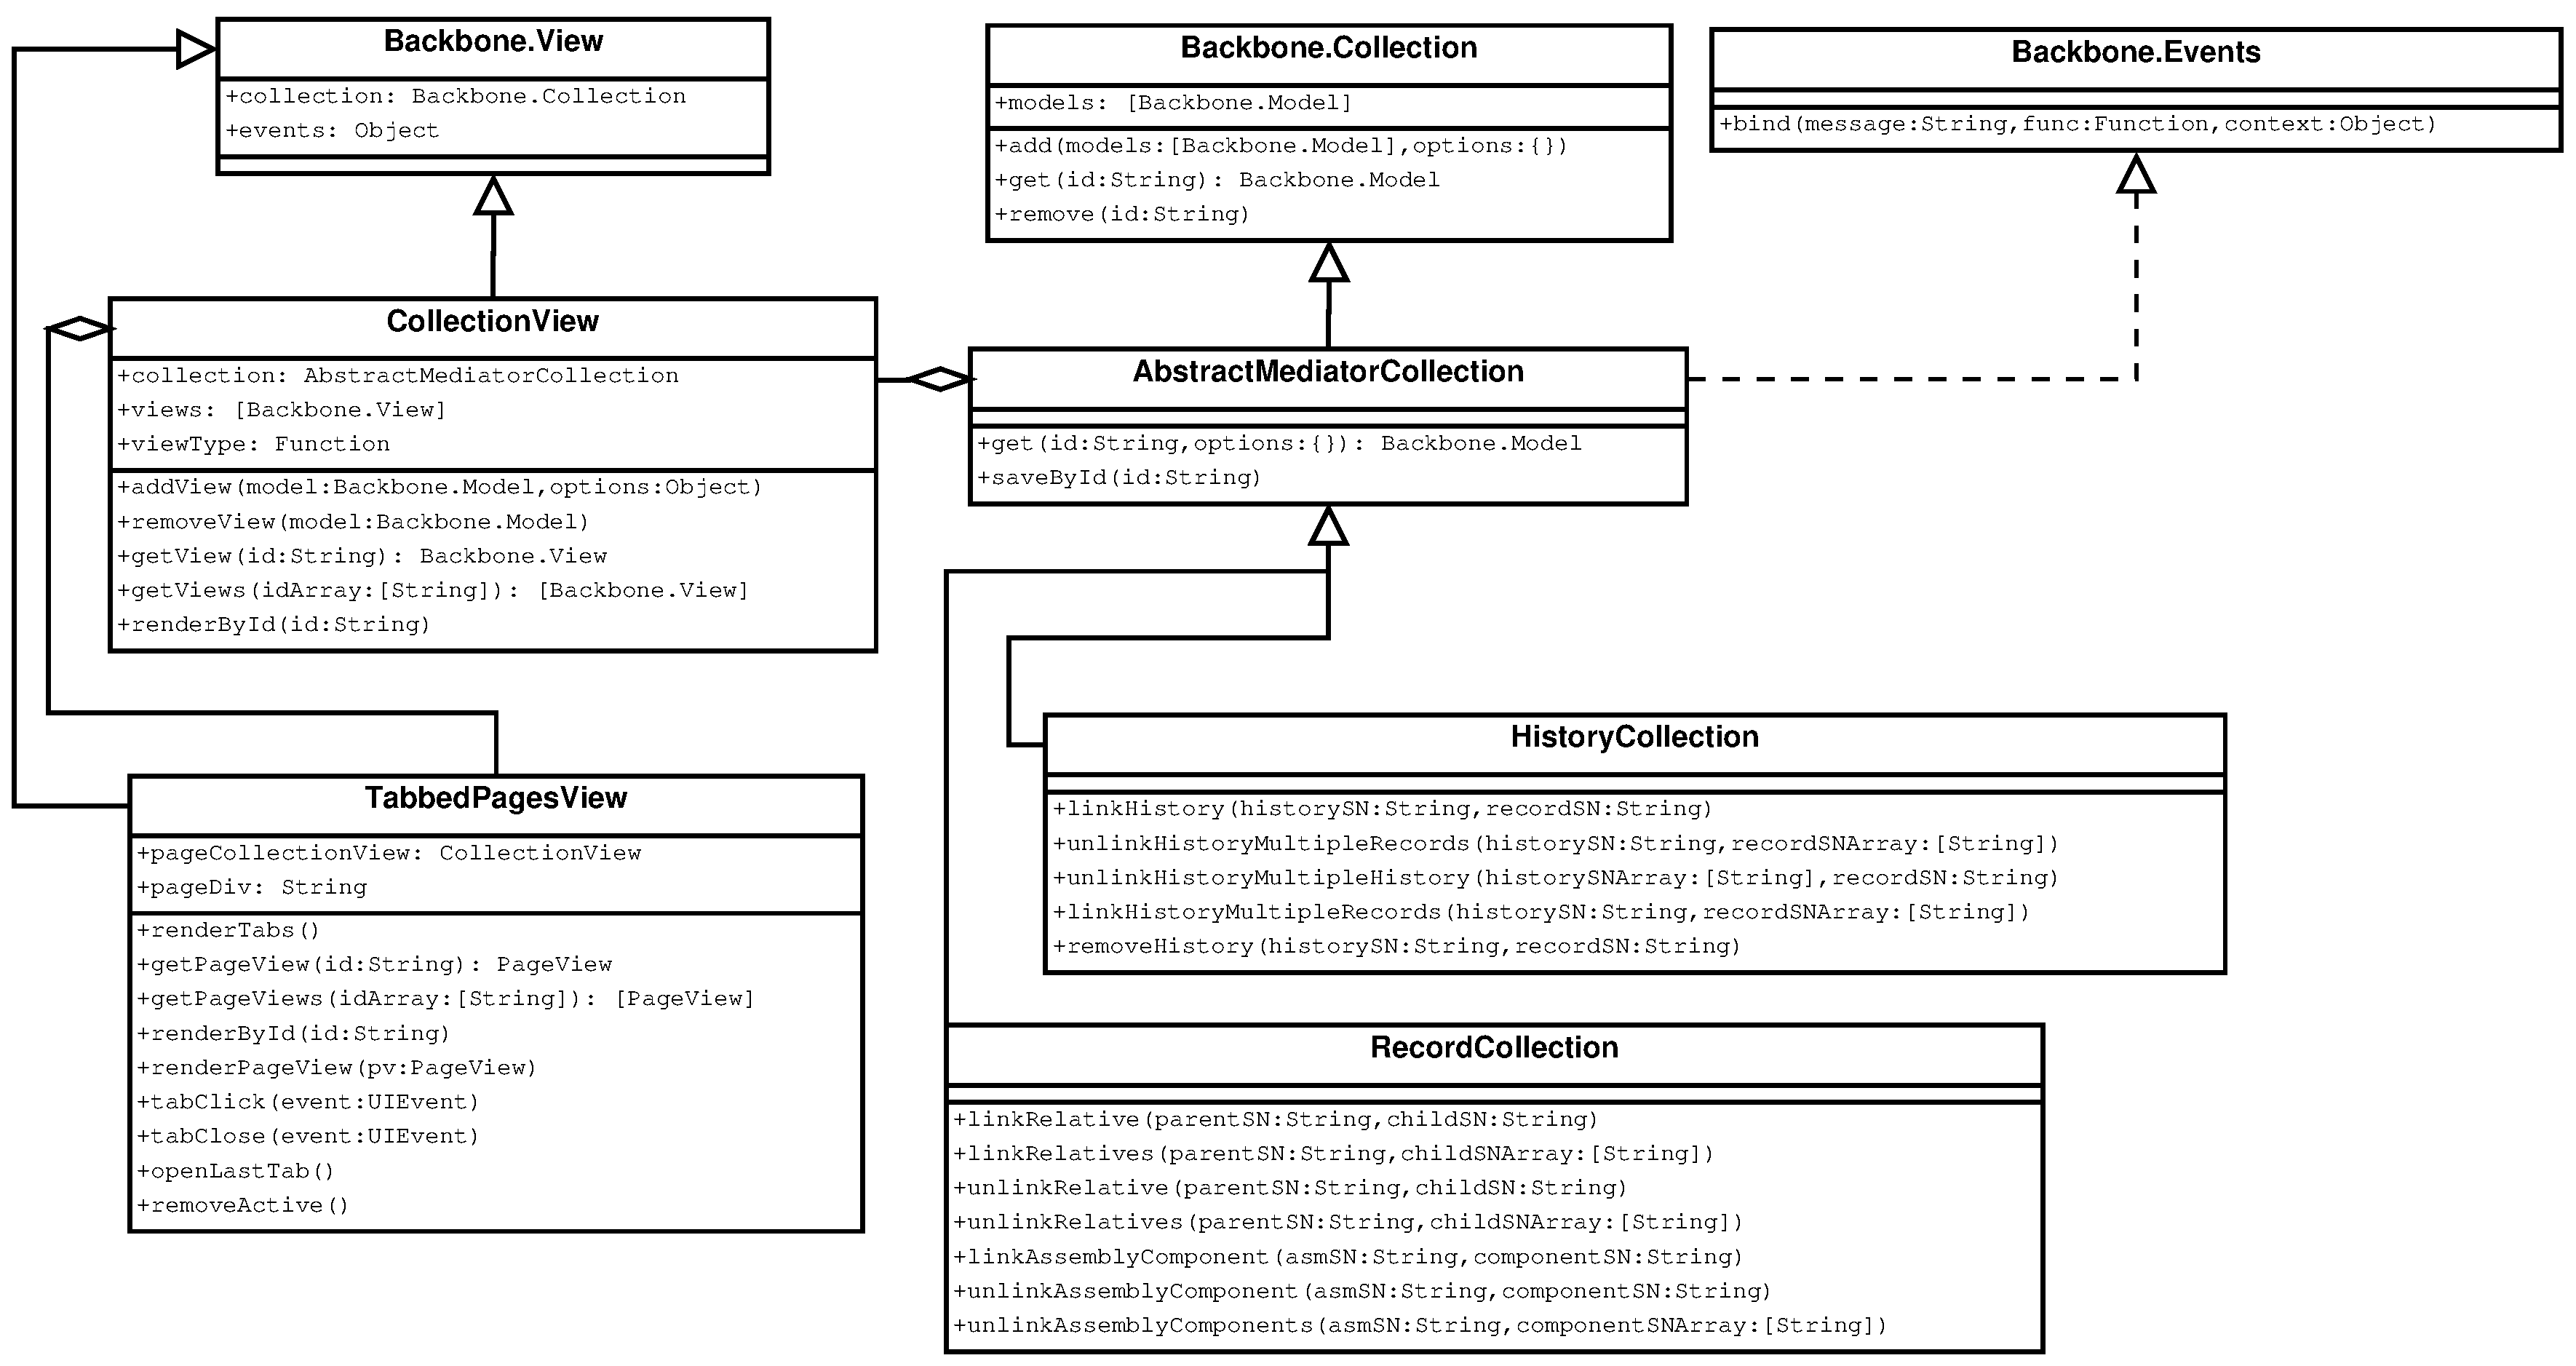
\includegraphics[height=3.75in]{Singletons}
\caption{A structure diagram of important Collection singletons and their associated views. CollectionViews aggregate views for models in
AbstractMediatorCollections. TabbedPagesView presents the tabbed page interface which is the primary point of interaction with users, and it
does so by manipulating an internal CollectionView. HistoryCollection and RecordCollection inherit properties from AbstractMediatorCollection
and act as mediators, controlling the logic that links relatives, assembly components, and history entries.}
\label{singletons}
\end{figure}

\begin{figure}[!p]
\centering
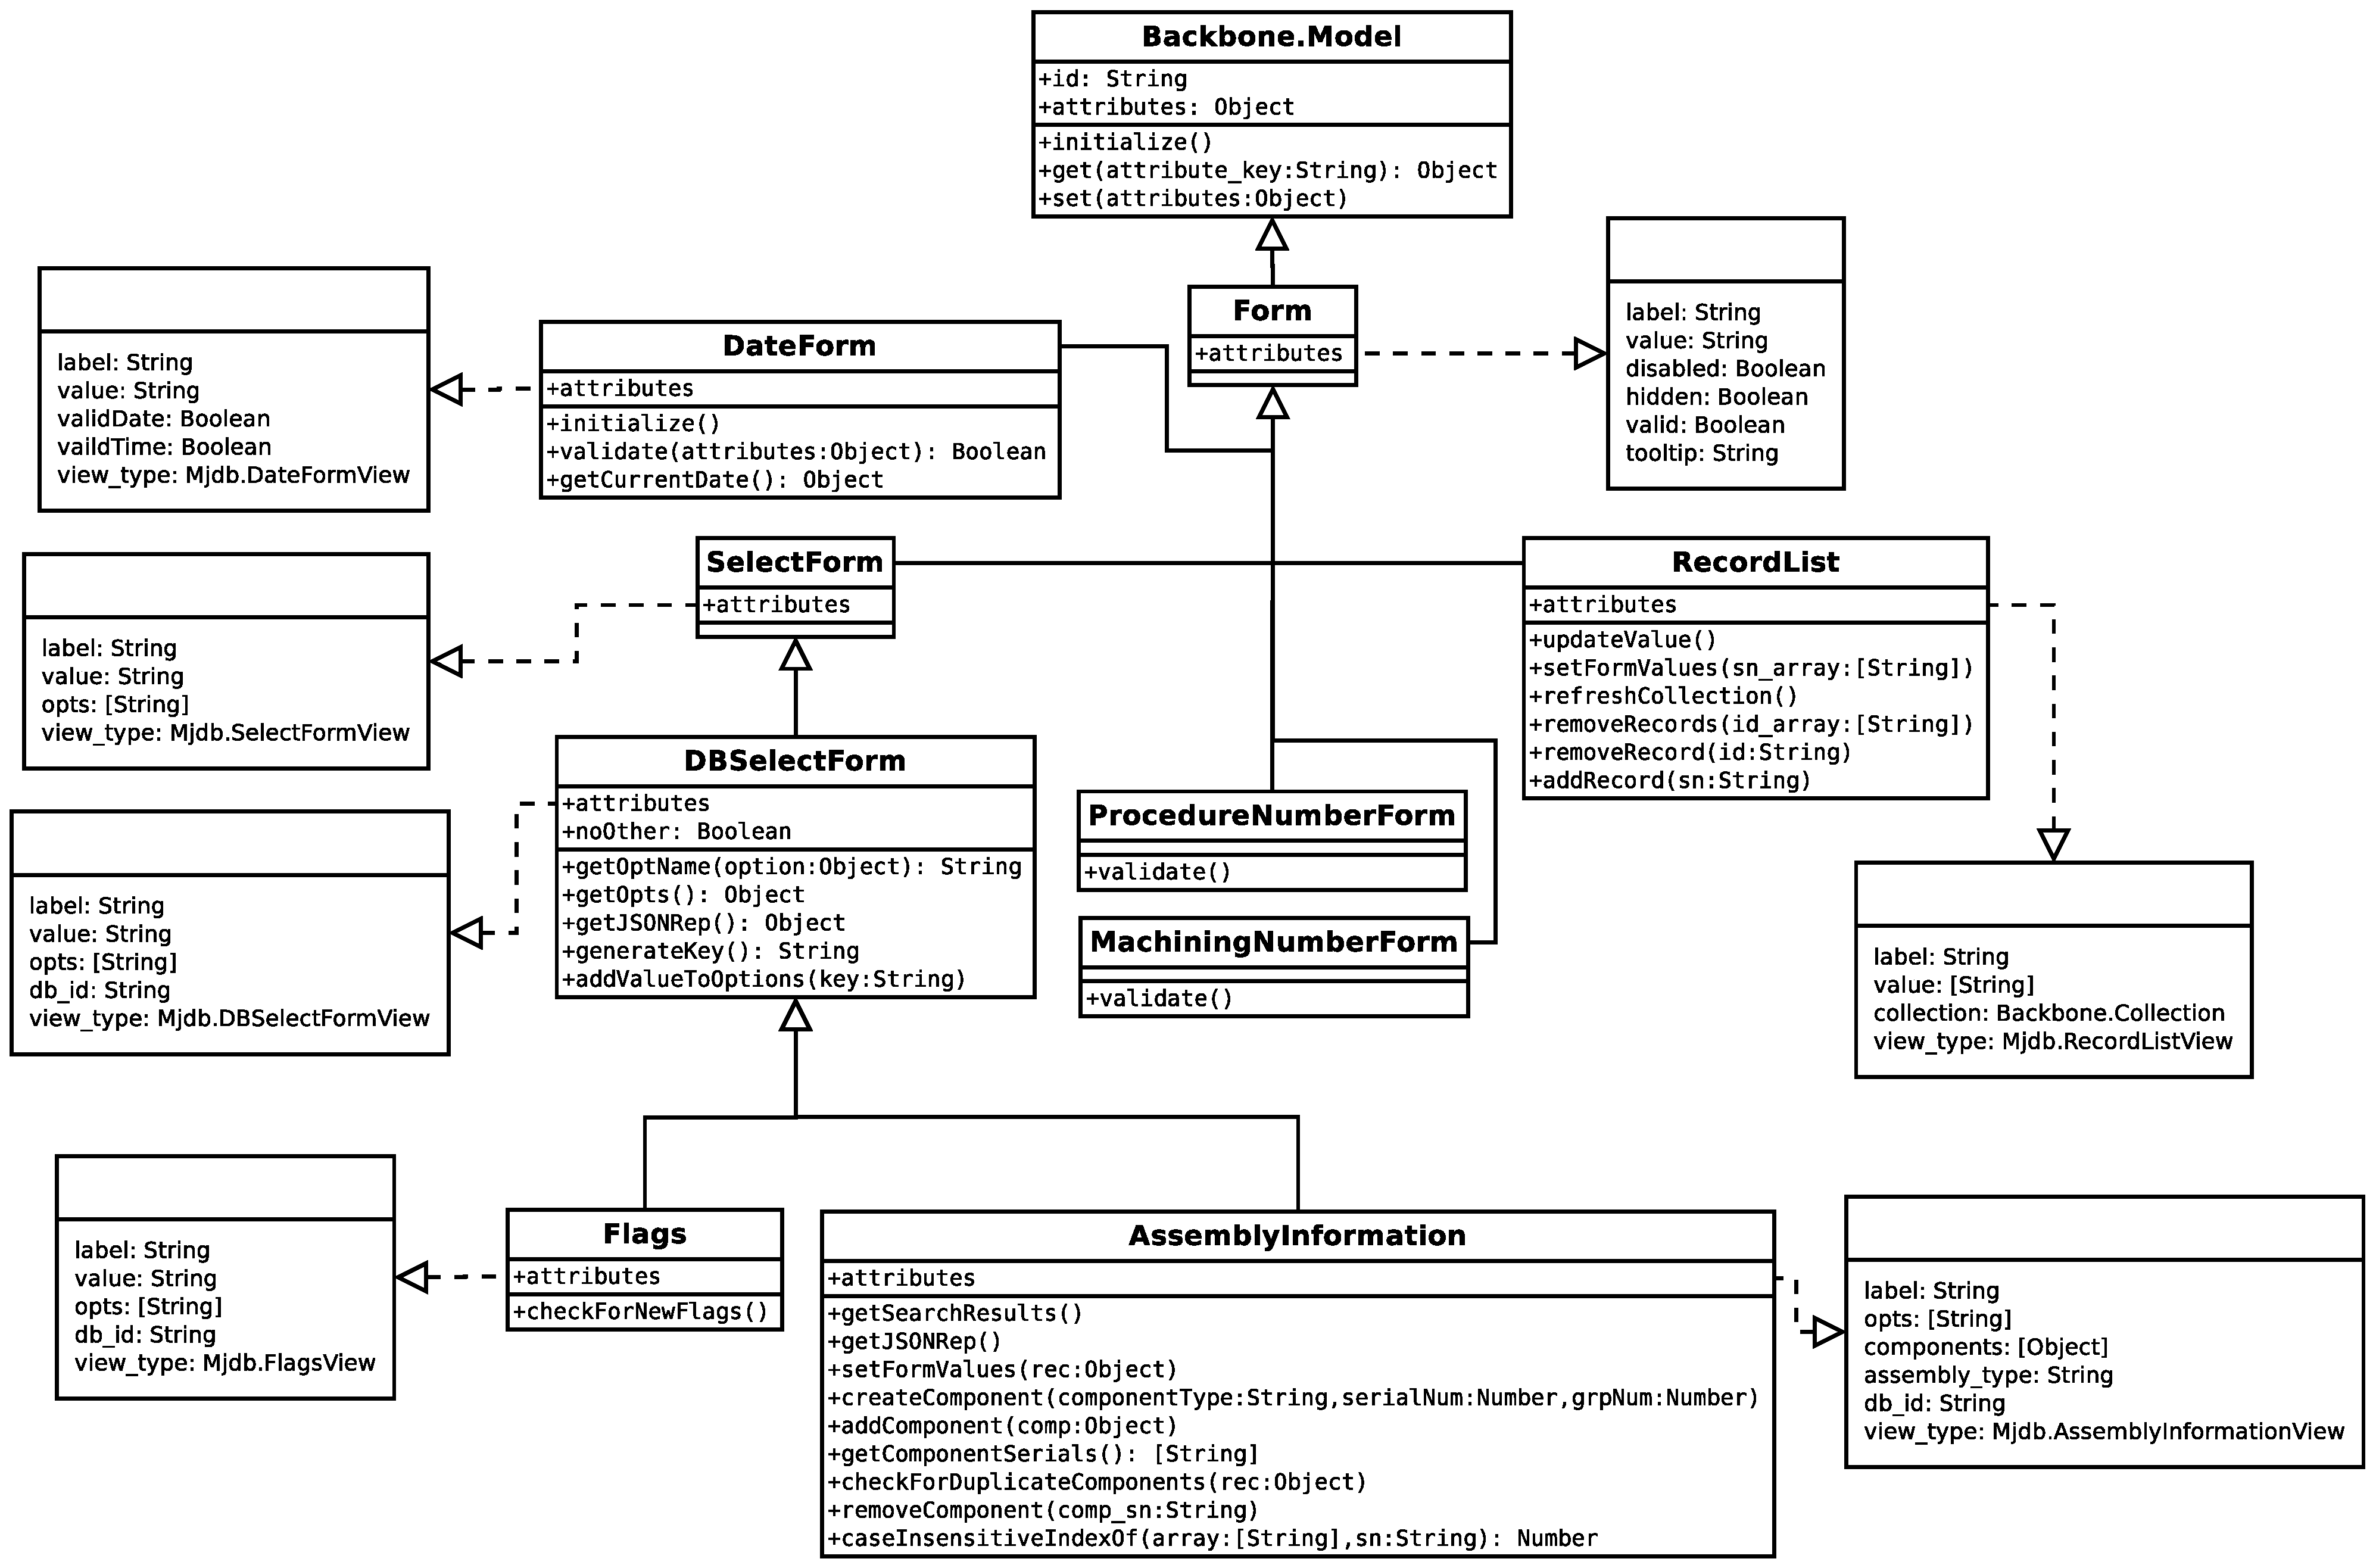
\includegraphics[height=3.75in]{Models}
\caption{The Form model inheritance tree. Each model has an attributes object containing the state of the model as well as the default
view type to be used by the FormCollectionView instance which presents the model to the user. The tree of FormView objects closely mirrors
the structure of the Form model tree.}
\label{models}
\end{figure}

\clearpage

% An example of a floating figure using the graphicx package.
% Note that \label must occur AFTER (or within) \caption.
% For figures, \caption should occur after the \includegraphics.
% Note that IEEEtran v1.7 and later has special internal code that
% is designed to preserve the operation of \label within \caption
% even when the captionsoff option is in effect. However, because
% of issues like this, it may be the safest practice to put all your
% \label just after \caption rather than within \caption{}.
%
% Reminder: the "draftcls" or "draftclsnofoot", not "draft", class
% option should be used if it is desired that the figures are to be
% displayed while in draft mode.
%
%\begin{figure}[!t]
%\centering
%\includegraphics[width=2.5in]{myfigure}
% where an .eps filename suffix will be assumed under latex, 
% and a .pdf suffix will be assumed for pdflatex; or what has been declared
% via \DeclareGraphicsExtensions.
%\caption{Simulation Results.}
%\label{fig_sim}
%\end{figure}

% Note that IEEE typically puts floats only at the top, even when this
% results in a large percentage of a column being occupied by floats.


% An example of a double column floating figure using two subfigures.
% (The subfig.sty package must be loaded for this to work.)
% The subfigure \label commands are set within each subfloat command,
% and the \label for the overall figure must come after \caption.
% \hfil is used as a separator to get equal spacing.
% Watch out that the combined width of all the subfigures on a 
% line do not exceed the text width or a line break will occur.
%
%\begin{figure*}[!t]
%\centering
%\subfloat[Case I]{\includegraphics[width=2.5in]{box}%
%\label{fig_first_case}}
%\hfil
%\subfloat[Case II]{\includegraphics[width=2.5in]{box}%
%\label{fig_second_case}}
%\caption{Simulation results.}
%\label{fig_sim}
%\end{figure*}
%
% Note that often IEEE papers with subfigures do not employ subfigure
% captions (using the optional argument to \subfloat[]), but instead will
% reference/describe all of them (a), (b), etc., within the main caption.


% An example of a floating table. Note that, for IEEE style tables, the 
% \caption command should come BEFORE the table. Table text will default to
% \footnotesize as IEEE normally uses this smaller font for tables.
% The \label must come after \caption as always.
%
%\begin{table}[!t]
%% increase table row spacing, adjust to taste
%\renewcommand{\arraystretch}{1.3}
% if using array.sty, it might be a good idea to tweak the value of
% \extrarowheight as needed to properly center the text within the cells
%\caption{An Example of a Table}
%\label{table_example}
%\centering
%% Some packages, such as MDW tools, offer better commands for making tables
%% than the plain LaTeX2e tabular which is used here.
%\begin{tabular}{|c||c|}
%\hline
%One & Two\\
%\hline
%Three & Four\\
%\hline
%\end{tabular}
%\end{table}


% Note that IEEE does not put floats in the very first column - or typically
% anywhere on the first page for that matter. Also, in-text middle ("here")
% positioning is not used. Most IEEE journals use top floats exclusively.
% Note that, LaTeX2e, unlike IEEE journals, places footnotes above bottom
% floats. This can be corrected via the \fnbelowfloat command of the
% stfloats package.

% if have a single appendix:
%\appendix[Proof of the Zonklar Equations]
% or
%\appendix  % for no appendix heading
% do not use \section anymore after \appendix, only \section*
% is possibly needed

% use appendices with more than one appendix
% then use \section to start each appendix
% you must declare a \section before using any
% \subsection or using \label (\appendices by itself
% starts a section numbered zero.)
%

\appendices
\section{Software Libraries Used in the PTDB}
\subsection{Web Application}
\begin{itemize}
  \item \textbf{JQuery} -- http://jquery.com/

   JQuery is a popular JavaScript library which simplifies 
   DOM interaction, AJAX requests, and simple UI effects.
   The JQuery UI toolkit is also used for the datepicker
   calendar functionality.
  \item \textbf{Underscore.js} -- http://underscorejs.org/

   Underscore is a JavaScript utility library used for common
   tasks and lending a functional programming style where
   desired.
   It is required by Backbone.js.
  \item \textbf{Backbone.js} -- http://backbonejs.org/

   Backbone.js provides a model-view decomposition by providing
   Model, View, and Collection prototype objects. It also provides
   a Sync object for database interactions as well as a Router object
   for URL fragment navigation and page history. 
\end{itemize}
\subsection{Exposure Calculator}
\begin{itemize}
  \item \textbf{Twisted} -- http://twistedmatrix.com/trac/

   Twisted is a Python network programming layer we use to serve
   JSON exposure data via HTTP. It is an event-driven library which
   turns URI requests into function execution, and returns data
   to the requester.
\end{itemize}

% use section* for acknowledgement
\section*{Acknowledgment}
The authors would like to thank the members of the \textsc{Majorana} collaboration
for their guidance while developing the PTDB software. Thanks also
to J. Esterline for his development contributions and help during testing.


% Can use something like this to put references on a page
% by themselves when using endfloat and the captionsoff option.
\ifCLASSOPTIONcaptionsoff
  \newpage
\fi



% trigger a \newpage just before the given reference
% number - used to balance the columns on the last page
% adjust value as needed - may need to be readjusted if
% the document is modified later
%\IEEEtriggeratref{8}
% The "triggered" command can be changed if desired:
%\IEEEtriggercmd{\enlargethispage{-5in}}

% references section

% can use a bibliography generated by BibTeX as a .bbl file
% BibTeX documentation can be easily obtained at:
% http://www.ctan.org/tex-archive/biblio/bibtex/contrib/doc/
% The IEEEtran BibTeX style support page is at:
% http://www.michaelshell.org/tex/ieeetran/bibtex/
\bibliographystyle{IEEEtran}
% argument is your BibTeX string definitions and bibliography database(s)
\bibliography{ksnavely_mjdb}

% biography section
% 
% If you have an EPS/PDF photo (graphicx package needed) extra braces are
% needed around the contents of the optional argument to biography to prevent
% the LaTeX parser from getting confused when it sees the complicated
% \includegraphics command within an optional argument. (You could create
% your own custom macro containing the \includegraphics command to make things
% simpler here.)
%\begin{IEEEbiography}[{\includegraphics[width=1in,height=1.25in,clip,keepaspectratio]{mshell}}]{Michael Shell}
% or if you just want to reserve a space for a photo:

% if you will not have a photo at all:
\begin{IEEEbiographynophoto}{John Doe}
Biography text here.
\end{IEEEbiographynophoto}

% You can push biographies down or up by placing
% a \vfill before or after them. The appropriate
% use of \vfill depends on what kind of text is
% on the last page and whether or not the columns
% are being equalized.

%\vfill

% Can be used to pull up biographies so that the bottom of the last one
% is flush with the other column.
%\enlargethispage{-5in}



% that's all folks
\end{document}


